%&tex

\chapter{Experiments and benchmarks}\label{chp:benchmarks}

In this chapter we apply our model on an artificial self-driving dataset, running several
experiments and measuring how good our models perform with each setup. The thinking behind this
benchmarking is to provide an initial screening to find the best SPN iteration to use on a
real-world testing scenario.

We first show results on accuracy for each of the models and pre-processing transformations.
We then show how fast each model is, i.e. how long it took for training and how much time it took
for the model to predict a label.

\section{Setups}

For our experiments, we tested two structure learning algorithms, the Dennis-Ventura and
Gens-Domingos architectures, and for each of these models we evaluated accuracy when applying
either generative or discriminative weight learning. We additionally ran tests without applying
weight learning to serve as reference. In this case, for the Gens-Domingos architecture we set
weights proportional to each cluster size, whereas in Dennis-Ventura we randomized weights.

For the Dennis-Ventura algorithm, we discarded pre-clustering, opting to use the classification
architecture mentioned in~\autoref{chp:structure}, as it resulted in much better accuracy. We also
fixed the number of sums per region and gaussians per pixel to four, and the similarity threshold
to $0.975$.

For the Gens-Domingos algorithm, we tested two implementations. The first uses $k$-means for the
clustering step with $k=2$. The second uses DBSCAN, with parameters $\epsilon=4$ the maximum radius
of a point neighborhood, and $m=4$ the minimum number of points to describe a dense region. Both
were set with a $p$-value of $0.01$ for the independence step. We refer to the $k$-means
implementation as $k$-GD, and the DBSCAN variation as DBSCAN-GD.
\begin{figure}[h]
  \centering
  \begin{tikzpicture}
    \node[inner sep=0pt, label=Raw] (raw) at (0, 0)
      {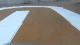
\includegraphics{imgs/pipe_raw.png}};
    \node[inner sep = 0pt, right = 2.0cm of raw, label=Gray] (gray)
      {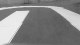
\includegraphics{imgs/pipe_gray.png}};
    \node[inner sep = 0pt, right = 2.0cm of gray, label=Binarized] (bin)
      {
\includegraphics{imgs/pipe_bin.png}};
    \node[rectangle, rounded corners, draw, below = 2.0cm of gray,
      minimum size=2cm] (weights) {LearnWeight};
    \node[rectangle, rounded corners, draw, right = 2.0cm of weights,
      minimum size=2cm] (struct) {LearnStructure};
    \node[cylinder, shape border rotate=90, draw, left = 2.0cm of weights,
      label=below:SaveDisk, minimum width=2cm, minimum height=1cm] (save) {};
    \node[inner sep = 0.75cm, rectangle, dashed, draw, thick, fit=(raw) (gray) (bin),
      label=above:\textbf{Pre-processing}] (pp) {};
    \node[inner sep = 0.5cm, rectangle, dotted, draw, thick, fit=(struct) (weights) (save),
      label=above:\textbf{Training}] (train) {};
    \draw[->,thick] (raw.east) -- (gray.west);
    \draw[->,thick] (gray.east) -- (bin.west);
    \draw[->,thick] let \p1 = (train.east), \p2 = (pp.east) in
      (\p2) -- ($ (\p2) + (0.5, 0) $) -- ($ (\x2, \y1) + (0.5, 0) $) -- (\p1);
    \draw[->,thick] (struct.west) -- (weights.east);
    \draw[->,thick] (weights.west) -- (save.east);
  \end{tikzpicture}
  \caption{Our training pipeline when using binarization in pre-processing.\label{fig:train_pipe}}
\end{figure}
DBSCAN-GD achieved the best scores, but took the longest time for both training and testing. We did
not test all possible iterations of pre-processing in this case, as DBSCAN-GD had too long training
times (an average of 10 hours for training alone). We found that when using DBSCAN-GD, the
resulting structure was too complex (about 32 times bigger than $k$-GD), causing inference to take
too long. For instance, when running inference on $k$-GD, average prediction took about $0.1$
second.  When using DBSCAN, the average time of prediction was $19.72$ seconds. However, in terms
of accuracy, DBSCAN-GD showed impressive results, with all tests achieving a perfect score of 100\%
accuracy. Despite these numbers, a model that takes too long for inference is not adequate for a
self-driving application. For this reason, we discarded the DBSCAN-GD model and decided to only use
the $k$-GD model.

In both training and testing, we first apply image transformations (e.g. quantizing, binarization
or equalization) to the dataset and then train or perform prediction with a particular model. The
applied image transformation is always identical in training and testing. For example, a valid
training pipeline would be choosing to apply 3-bit quantization and equalization to a training
dataset, train an SPN structure using $k$-GD, perform discriminative gradient descent on the
resulting structure to learn its weights, and finally save the model for testing. Its then
equivalent testing pipeline would be applying the same image transformation, in our case 3-bit
quantization and equalization, and for each image find the $\argmax_{y\in Y} P(Y=y|X)$.
\autoref{fig:train_pipe} shows a visualization of the training pipeline, whereas
\autoref{fig:infer_pipe} displays its equivalent inference pipeline.

Both Gens-Domingos and Dennis-Ventura algorithms generate a structure as deep as the number of
training samples. The deeper the structure, the more expressive it is. We found that accuracy with
models trained with 1000 samples had much better accuracies than with 500. However, a more complex
network means inference will take longer. We attempted to keep inference at less than a second per
prediction. A training set size of 500 was chosen as the generated SPNs had decent prediction time
and accuracy, and did not take too long in training. The size of the testing dataset was also 500
images.

We use a particular set of notations for our experiments. For image transformations, we denote by
$Q_n$ as applying an $n$-bit quantization of the dataset. An $E$ means the dataset was equalized,
and a $B$ means it was binarized. Any combination of image transformation is signalled with a $+$
sign. A $\emptyset$ means there were no image transformations done to the dataset apart from
grayscale conversion.
\begin{figure}[h]
  \centering
  \begin{tikzpicture}
    \node[inner sep=0pt, label=Raw] (raw) at (0, 0)
      {
\includegraphics{imgs/pipe_out_raw.png}};
    \node[inner sep = 0pt, right = 2.0cm of raw, label=Gray] (gray)
      {
\includegraphics{imgs/pipe_out_gray.png}};
    \node[inner sep = 0pt, right = 2.0cm of gray, label=Binarized] (bin)
      {
\includegraphics{imgs/pipe_out_bin.png}};
    \node[inner sep = 0.75cm, rectangle, dashed, draw, thick, fit=(raw) (gray) (bin),
      label=above:\textbf{Pre-processing}] (pp) {};
    \node[cylinder, shape border rotate=90, draw, below = 2.0cm of raw,
      label=below:LoadDisk, minimum width=2cm, minimum height = 1cm] (load) {};
    \node[rectangle, rounded corners, draw, right = 2.0cm of load,
      minimum size=2cm] (build) {BuildSPN};
    \node[rectangle, rounded corners, draw, right = 2.0cm of build, right = 3.0cm of build,
      minimum size=2cm] (infer) {Inference};
    \node[inner sep = 0.5cm, rectangle, dotted, draw, thick, fit=(load) (build),
      label=below:\textbf{SPN loading}] (create) {};
    \node[below = 1.0cm of infer] (pred) {Predicted: RIGHT};
    \draw[->,thick] (raw.east) -- (gray.west);
    \draw[->,thick] (gray.east) -- (bin.west);
    \draw[->,thick] let \p1 = (infer.east), \p2 = (pp.east) in
      (\p2) -- ($ (\p2) + (0.5, 0) $) -- ($ (\x2, \y1) + (0.5, 0) $) -- (\p1);
    \draw[->,thick] (load) -- (build);
    \draw[->,thick] (create) -- (infer);
    \draw[->,thick] (infer) -- (pred);
  \end{tikzpicture}
  \caption{Our inference pipeline when using binarization in pre-processing.\label{fig:infer_pipe}}
\end{figure}

For learning algorithms, a GD means we are using $k$-means Gens-Domingos and DV Dennis-Ventura.
This is then followed by the weight learning algorithm used. The letters g, d and s mean we either
applied generative gradient descent, discriminative gradient descent or no weight learning.

Parameters for weight learning were fixed to learning rate $\eta=1.0$, L2 regularization constant
$\lambda=0.001$, mini-batch size $b=50$ and number of epochs $N=15$. In all setups weight learning
suffered heavily from gradient diffusion when using soft gradient descent, leading us to be forced
to only use hard gradient descent for all test.

\section{Accuracy}

In this section we show accuracy results in each setup. All values are in percentage of hits.

\begin{table}[h]
  \centering
  \begin{tabular}{l|c|c|c|c|c|c}
    \hline
    \multicolumn{1}{c}{\bfseries Accuracy (\%)} & \multicolumn{1}{c}{\bfseries DV+g} &
    \multicolumn{1}{c}{\bfseries DV+d} & \multicolumn{1}{c}{\bfseries DV+s} &
    \multicolumn{1}{c}{\bfseries GD+g} & \multicolumn{1}{c}{\bfseries GD+d} &
    \multicolumn{1}{c}{\bfseries GD+s}\\
    \hline
    $B$         & 78.8 & 78.8 & 78.8 & 82.8 & 83.8 & 85.0\\
    $Q_2$       & 78.6 & 78.0 & 78.0 & 78.6 & 80.4 & 79.4\\
    $Q_2+E$     & 76.6 & 76.6 & 76.8 & 79.6 & 82.8 & 81.8\\
    $Q_3$       & 77.4 & 77.4 & 77.4 & 77.6 & 80.2 & 79.8\\
    $Q_3+E$     & 70.4 & 76.6 & 76.6 & 79.2 & 81.2 & 77.4\\
    $Q_4$       & 78.2 & 78.4 & 78.2 & 76.0 & 78.2 & 76.4\\
    $Q_4+E$     & 76.6 & 76.6 & 76.8 & 76.0 & 74.6 & 80.6\\
    $Q_5$       & 77.8 & 78.4 & 78.4 & 77.6 & 74.0 & 73.8\\
    $Q_5+E$     & 76.6 & 76.6 & 76.6 & 72.0 & 72.8 & 72.0\\
    $Q_6$       & 77.4 & 78.4 & 78.4 & 75.2 & 74.4 & 72.0\\
    $Q_6+E$     & 76.0 & 76.4 & 76.4 & 73.0 & 75.0 & 73.6\\
    $Q_7$       & 78.2 & 78.4 & 78.4 & 62.8 & 72.2 & 71.4\\
    $Q_7+E$     & 76.2 & 76.4 & 76.4 & 70.6 & 71.4 & 71.6\\
    $\emptyset$ & 78.0 & 78.4 & 78.4 & 62.4 & 62.4 & 62.4\\
    $E$         & 76.4 & 76.4 & 76.4 & 60.4 & 60.0 & 61.2\\
  \end{tabular}
  \caption{Accuracy values for each possible model permutation.\label{tab:accuracy}}
\end{table}

\autoref{tab:accuracy} shows some interesting results. The first is that generative gradient
descent on the Dennis-Ventura architecture had a negative impact on the performance of
the network. Discriminative learning on the other hand seemed to not impact on accuracy at all. Not
only that, quantization seems to have no impact, with equalization always deteriorating accuracy.

The Gens-Domingos architecture, on the other hand, achieved better results, but showed a more
unpredictable behavior. When resolution was low, as is the case of $B$, $Q_2$ and $Q_3$, the GD
architecture seems to always outclass DV. In fact, our best results were, as expected, when we used
binarization, as we're only tracking the most significant feature: lane bounds. In some cases
generative learning improved accuracy, but in most cases it had a negative impact.  Discriminative
learning, on the other hand, seemed to usually enhance the network's accuracy.

Our main takeaway from these accuracy results is that the structure of an SPN is much more
meaningful than its weights. Generative learning in our use case had a negative impact, and
discriminative learning usually provides a small boost to accuracy.

\section{Speed}

In this section we try to quantify both training and inference of our models in each setup. We ran
all tests on an Intel Core i7-4500U CPU @ 1.8GHz, a 2-core 4-threaded processor. For memory we had
16GB RAM and 16GB swap space, though training didn't use more than 4GB and testing didn't exceed
100MB.

\begin{table}[h]
  \centering
  \begin{tabular}{l|c|c|c|c|c|c}
    \hline
    \multicolumn{1}{c}{\bfseries Training (mins)} & \multicolumn{1}{c}{\bfseries DV+g} &
    \multicolumn{1}{c}{\bfseries DV+d} & \multicolumn{1}{c}{\bfseries DV+s} &
    \multicolumn{1}{c}{\bfseries GD+g} & \multicolumn{1}{c}{\bfseries GD+d} &
    \multicolumn{1}{c}{\bfseries GD+s}\\
    \hline
    $B$         & 22m36s & 34m23s & 01m03s & 85m58s & 200m53s& 01m50s \\
    $Q_2$       & 22m07s & 34m59s & 00m23s & 52m57s & 125m17s& 01m28s \\
    $Q_2+E$     & 22m01s & 35m05s & 00m24s & 98m51s & 232m20s& 09m36s \\
    $Q_3$       & 22m15s & 32m42s & 00m25s & 34m24s & 96m18s & 04m56s \\
    $Q_3+E$     & 22m25s & 32m35s & 00m25s & 44m47s & 102m03s& 13m01s \\
    $Q_4$       & 22m16s & 31m56s & 00m25s & 31m25s & 41m46s & 08m15s \\
    $Q_4+E$     & 22m23s & 31m49s & 00m31s & 34m21s & 45m42s & 11m35s \\
    $Q_5$       & 22m24s & 35m06s & 00m29s & 23m10s & 23m18s & 07m24s \\
    $Q_5+E$     & 22m25s & 36m44s & 00m29s & 20m13s & 29m38s & 08m36s \\
    $Q_6$       & 22m20s & 36m34s & 00m27s & 49m22s & 50m35s & 21m37s \\
    $Q_6+E$     & 22m12s & 37m13s & 00m27s & 54m53s & 43m30s & 21m17s \\
    $Q_7$       & 22m13s & 33m14s & 00m30s & 78m05s & 72m03s & 43m44s \\
    $Q_7+E$     & 22m22s & 37m40s & 00m29s & 95m30s & 79m48s & 65m19s \\
    $\emptyset$ & 22m10s & 36m56s & 00m33s &166m53s & 107m44s& 90m22s \\
    $E$         & 22m10s & 34m58s & 00m33s &174m55s & 116m41s& 186m49s\\
  \end{tabular}
  \caption{Average time in minutes and seconds for training each model.\label{tab:time-training}}
\end{table}

Training time for DV was very well behaved, as~\autoref{tab:time-training} shows. As expected,
discriminative gradient descent took the most time, as we require two passes through the network
for each mini-batch.

Training time with gradient descent depends on the depth of the network. We found that the DV
structure had very regular training times for only generating the network. Not only that,
regardless of pre-processing the network had very similar network depth and size. This was in clear
distinction with the Gens-Domingos structure. In fact, binarization generated the deepest network,
whilst training the structure with no pre-processing resulted in the shallowest. Interestingly,
on average, deeper networks took the least time to train and had the best accuracy results. This is
probably due to better variable partitioning during the independence step, resulting in a better
balanced and more expressive tree.

\autoref{tab:time-inference} shows how much time it took, on average, to predict a single image.
Computation of the average time was done by timing all 500 predictions on the test dataset, and
then dividing by the number of total predictions.  Again, the DV architecture had very regular
times. The GD structure, on the other hand, showed how much deeper the SPN structures are with
heavy quantization.

\begin{table}[h]
  \centering
  \begin{tabular}{l|c|c|c|c|c|c}
    \hline
    \multicolumn{1}{c}{\bfseries Inference (secs)} & \multicolumn{1}{c}{\bfseries DV+g} &
    \multicolumn{1}{c}{\bfseries DV+d} & \multicolumn{1}{c}{\bfseries DV+s} &
    \multicolumn{1}{c}{\bfseries GD+g} & \multicolumn{1}{c}{\bfseries GD+d} &
    \multicolumn{1}{c}{\bfseries GD+s}\\
    \hline
    $B$         & 0.23 & 0.25 & 0.25 & 0.38 & 0.37 & 0.31 \\
    $Q_2$       & 0.22 & 0.24 & 0.23 & 0.28 & 0.34 & 0.16 \\
    $Q_2+E$     & 0.22 & 0.23 & 0.23 & 0.38 & 0.30 & 0.27 \\
    $Q_3$       & 0.22 & 0.23 & 0.22 & 0.22 & 0.32 & 0.17 \\
    $Q_3+E$     & 0.22 & 0.23 & 0.22 & 0.34 & 0.32 & 0.31 \\
    $Q_4$       & 0.22 & 0.22 & 0.23 & 0.16 & 0.17 & 0.13 \\
    $Q_4+E$     & 0.23 & 0.27 & 0.29 & 0.13 & 0.14 & 0.13 \\
    $Q_5$       & 0.22 & 0.26 & 0.28 & 0.07 & 0.05 & 0.02 \\
    $Q_5+E$     & 0.22 & 0.29 & 0.25 & 0.05 & 0.05 & 0.02 \\
    $Q_6$       & 0.23 & 0.24 & 0.23 & 0.04 & 0.05 & 0.01 \\
    $Q_6+E$     & 0.22 & 0.24 & 0.28 & 0.03 & 0.04 & 0.02 \\
    $Q_7$       & 0.23 & 0.23 & 0.26 & 0.03 & 0.01 & 0.01 \\
    $Q_7+E$     & 0.22 & 0.26 & 0.24 & 0.01 & 0.01 & 0.01 \\
    $\emptyset$ & 0.22 & 0.26 & 0.23 & 0.02 & 0.01 & 0.01 \\
    $E$         & 0.23 & 0.23 & 0.22 & 0.01 & 0.01 & 0.02 \\
  \end{tabular}
  \caption{Average time in seconds to predict a single image.\label{tab:time-inference}}
\end{table}
